\documentclass[conference]{IEEEtran}

\usepackage{amsmath,amssymb,amsfonts}
\usepackage{algorithmic}
\usepackage{graphicx}
\usepackage{textcomp}
\usepackage{xcolor}
\usepackage{booktabs}
\usepackage{tabularx}
\usepackage{array}
\usepackage{url}
\usepackage{cite}
\usepackage{multirow}
\usepackage{subcaption}
\usepackage{listings}

% Configure listings for Python snippets
\lstset{
  basicstyle=\ttfamily\scriptsize,
  keywordstyle=\color{blue}\bfseries,
  stringstyle=\color{red!70!black},
  commentstyle=\color{green!50!black}\itshape,
  numbers=left,
  numberstyle=\tiny\color{gray},
  stepnumber=1,
  numbersep=4pt,
  backgroundcolor=\color{gray!8},
  showspaces=false,
  showstringspaces=false,
  showtabs=false,
  frame=single,
  rulecolor=\color{gray!30},
  tabsize=2,
  captionpos=b,
  breaklines=true,
  breakatwhitespace=false
}

% Graphics path
\graphicspath{{figures/}}

\title{Autonomous Data Science Analyst Agent: A Deterministic LangGraph Orchestration Framework for End-to-End Automated Machine Learning and Explainable Text Classification}

\author{\IEEEauthorblockN{Vaibhav Bhagat}
\IEEEauthorblockA{\textit{Department of Computer Science and Engineering} \\
\textit{Affiliated Engineering Institution}\\
Email: author@institution.edu}
\and
\IEEEauthorblockN{Co-Author Name}
\IEEEauthorblockA{\textit{Department of Computer Science and Engineering} \\
\textit{Affiliated Engineering Institution}\\
Email: coauthor@institution.edu}
}

\begin{document}
\maketitle

\begin{abstract}
While Automated Machine Learning (AutoML) frameworks have reduced engineering friction in hyperparameter optimization and algorithm selection, the end-to-end data science lifecycle remains severely fragmented. Real-world analytical practitioners spend up to 70\% of operational bandwidth manually writing boilerplate code for file schema profiling, corrupted anomaly cleaning, exploratory visual analysis, explainable metric extraction, and deployment-ready artifact packaging. Conversely, emergent Large Language Model (LLM) autonomous code-interpreters suffer from ungrounded hallucination of tabular schemas, runtime execution loops, and unacceptable cloud data-privacy leaks. To systematically resolve these limitations, this paper presents the \textit{Autonomous Data Science Analyst Agent}, a novel multi-agent state-machine system coordinated via a directed acyclic LangGraph architecture. The framework establishes a strict separation of concerns: deterministic Python-based computational agents handle schema profiling, singleton noise pruning, and scikit-learn feature modeling, while an isolated LLM agent (executed via local Qwen3-14B or cloud Gemini) functions exclusively as a high-level goal orchestrator constrained by Pydantic-typed validation boundaries. When benchmarked on the classic 5,573-sample SMS/Email Spam corpus, the system autonomously identifies and rectifies 415 exact record duplicates and eliminates singleton malformed classes, constructing a competitive TF-IDF feature pipeline yielding 97.48\% test accuracy, 97.42\% weighted F1-score, and transparent coefficient-based feature explanations without any human intervention in under 3.2 seconds.
\end{abstract}

\begin{IEEEkeywords}
Automated Machine Learning, Multi-Agent Systems, LangGraph, Large Language Models, Text Classification, Explainable Artificial Intelligence, Deterministic State Machines.
\end{IEEEkeywords}

\section{Introduction}
\IEEEPARstart{T}{he} contemporary lifecycle of experimental data science is characterized by severe operational fragmentation. Building production-grade machine learning classifiers requires data scientists to navigate multiple heterogeneous disciplines: structural schema profiling, tabular parsing, anomaly and duplicate cleansing, exploratory distribution visualization, high-dimensional feature engineering, dual-model cross-validation, Explainable AI (XAI) feature attribution, and final model serialization for web-dashboard consumption \cite{hutter2019automl, he2021automl}. Empirical studies consistently reveal that data practitioners spend upwards of 60\% to 70\% of their project lifecycles on repetitive, non-cognitive data wrangling and boilerplate script coordination rather than structural modeling \cite{munpy2020}.

To mitigate this bottleneck, Automated Machine Learning (AutoML) platforms such as Auto-Sklearn, TPOT, and H2O AutoML have automated portions of algorithm selection and hyperparameter optimization \cite{feurer2015autosklearn, olson2016tpot}. However, traditional AutoML frameworks operate predominantly as black-box optimizers. They lack semantic comprehension of user intent expressed in natural language, cannot dynamically generate contextual exploratory visual reports, and fail to provide end-to-end integration across data cleaning, explainability, and consumer-facing prediction interfaces.

With the recent proliferation of Large Language Models (LLMs) and autonomous agent frameworks, researchers have investigated generative AI for data science automation (e.g., CodeInterpreter, DS-Agent, ChatDev) \cite{hong2023metagpt, guo2024dsagent}. Nevertheless, unconstrained LLM code execution introduces critical vulnerabilities:
\begin{enumerate}
    \item \textbf{Schema Hallucination}: LLMs tasked with reading raw dataset bytes routinely hallucinate non-existent column names, data types, and target distributions, resulting in runtime execution failures.
    \item \textbf{Data Privacy Breaches}: Commercial cloud-based LLM APIs require sending proprietary enterprise datasets over public internet endpoints, directly violating strict corporate and regulatory compliance standards (e.g., GDPR, HIPAA).
    \item \textbf{Fragility Against Data Anomalies}: Real-world tabular datasets frequently contain severe class imbalances, unstripped carriage returns, and corrupt singleton target labels (single records with malformed strings) that crash standard stratified splitting algorithms during model cross-validation.
    \item \textbf{Black-Box Reasoning}: Pure prompt-driven systems fail to provide deterministic, reproducible audit logs and model explainability metrics.
\end{enumerate}

To bridge this fundamental research gap, we introduce the \textbf{Autonomous Data Science Analyst Agent}. The proposed system integrates a deterministic, state-machine orchestration backbone implemented via LangGraph \cite{langgraphdocs} with strict Pydantic-typed schema validation \cite{pydantic2023} and a privacy-preserving dual-LLM execution layer. The framework coordinates seven specialized functional agents across a robust Directed Acyclic Graph (DAG): Ingestion and Profiling, Structured Orchestration, Data Cleaning, Exploratory Data Analysis (EDA), Model Selection and Training, Explainability Attribution, and Synthesis Reporting.

\subsection{Key Scientific Contributions}
This research provides the following primary contributions:
\begin{itemize}
    \item \textbf{Deterministic Multi-Agent State Architecture}: We propose a novel state-machine framework using LangGraph and a typed \texttt{AnalystState} container that decouples high-level semantic reasoning from deterministic algorithmic execution, preventing recursive agent loops and ungrounded execution states.
    \item \textbf{Anti-Hallucination Schema Grounding}: We enforce strict Pydantic v2 structured output validation where LLM planning agents are mathematically restricted to select targets and operations exclusively from verified, pre-computed dataset profiles.
    \item \textbf{Privacy-Preserving Hybrid Inference}: The system provides native architectural support for local OpenAI-compatible endpoints (specifically Qwen3-14B executed via local runtimes), allowing 100\% offline dataset processing without compromising corporate privacy.
    \item \textbf{Comprehensive Noise \& Singleton Handling}: We design an automated sanitization protocol that automatically prunes exact message duplicates and filters malformed singleton target classes before stratified dataset splitting.
    \item \textbf{Empirical Validation \& Production Packaging}: We provide an end-to-end evaluation on the benchmark SMS Spam dataset, demonstrating competitive TF-IDF LinearSVC training (97.48\% accuracy, 97.42\% F1), transparent coefficient feature extraction, and automated delivery to a Streamlit interactive sandbox in under 3.2 seconds.
\end{itemize}

\begin{figure*}[t]
\centering
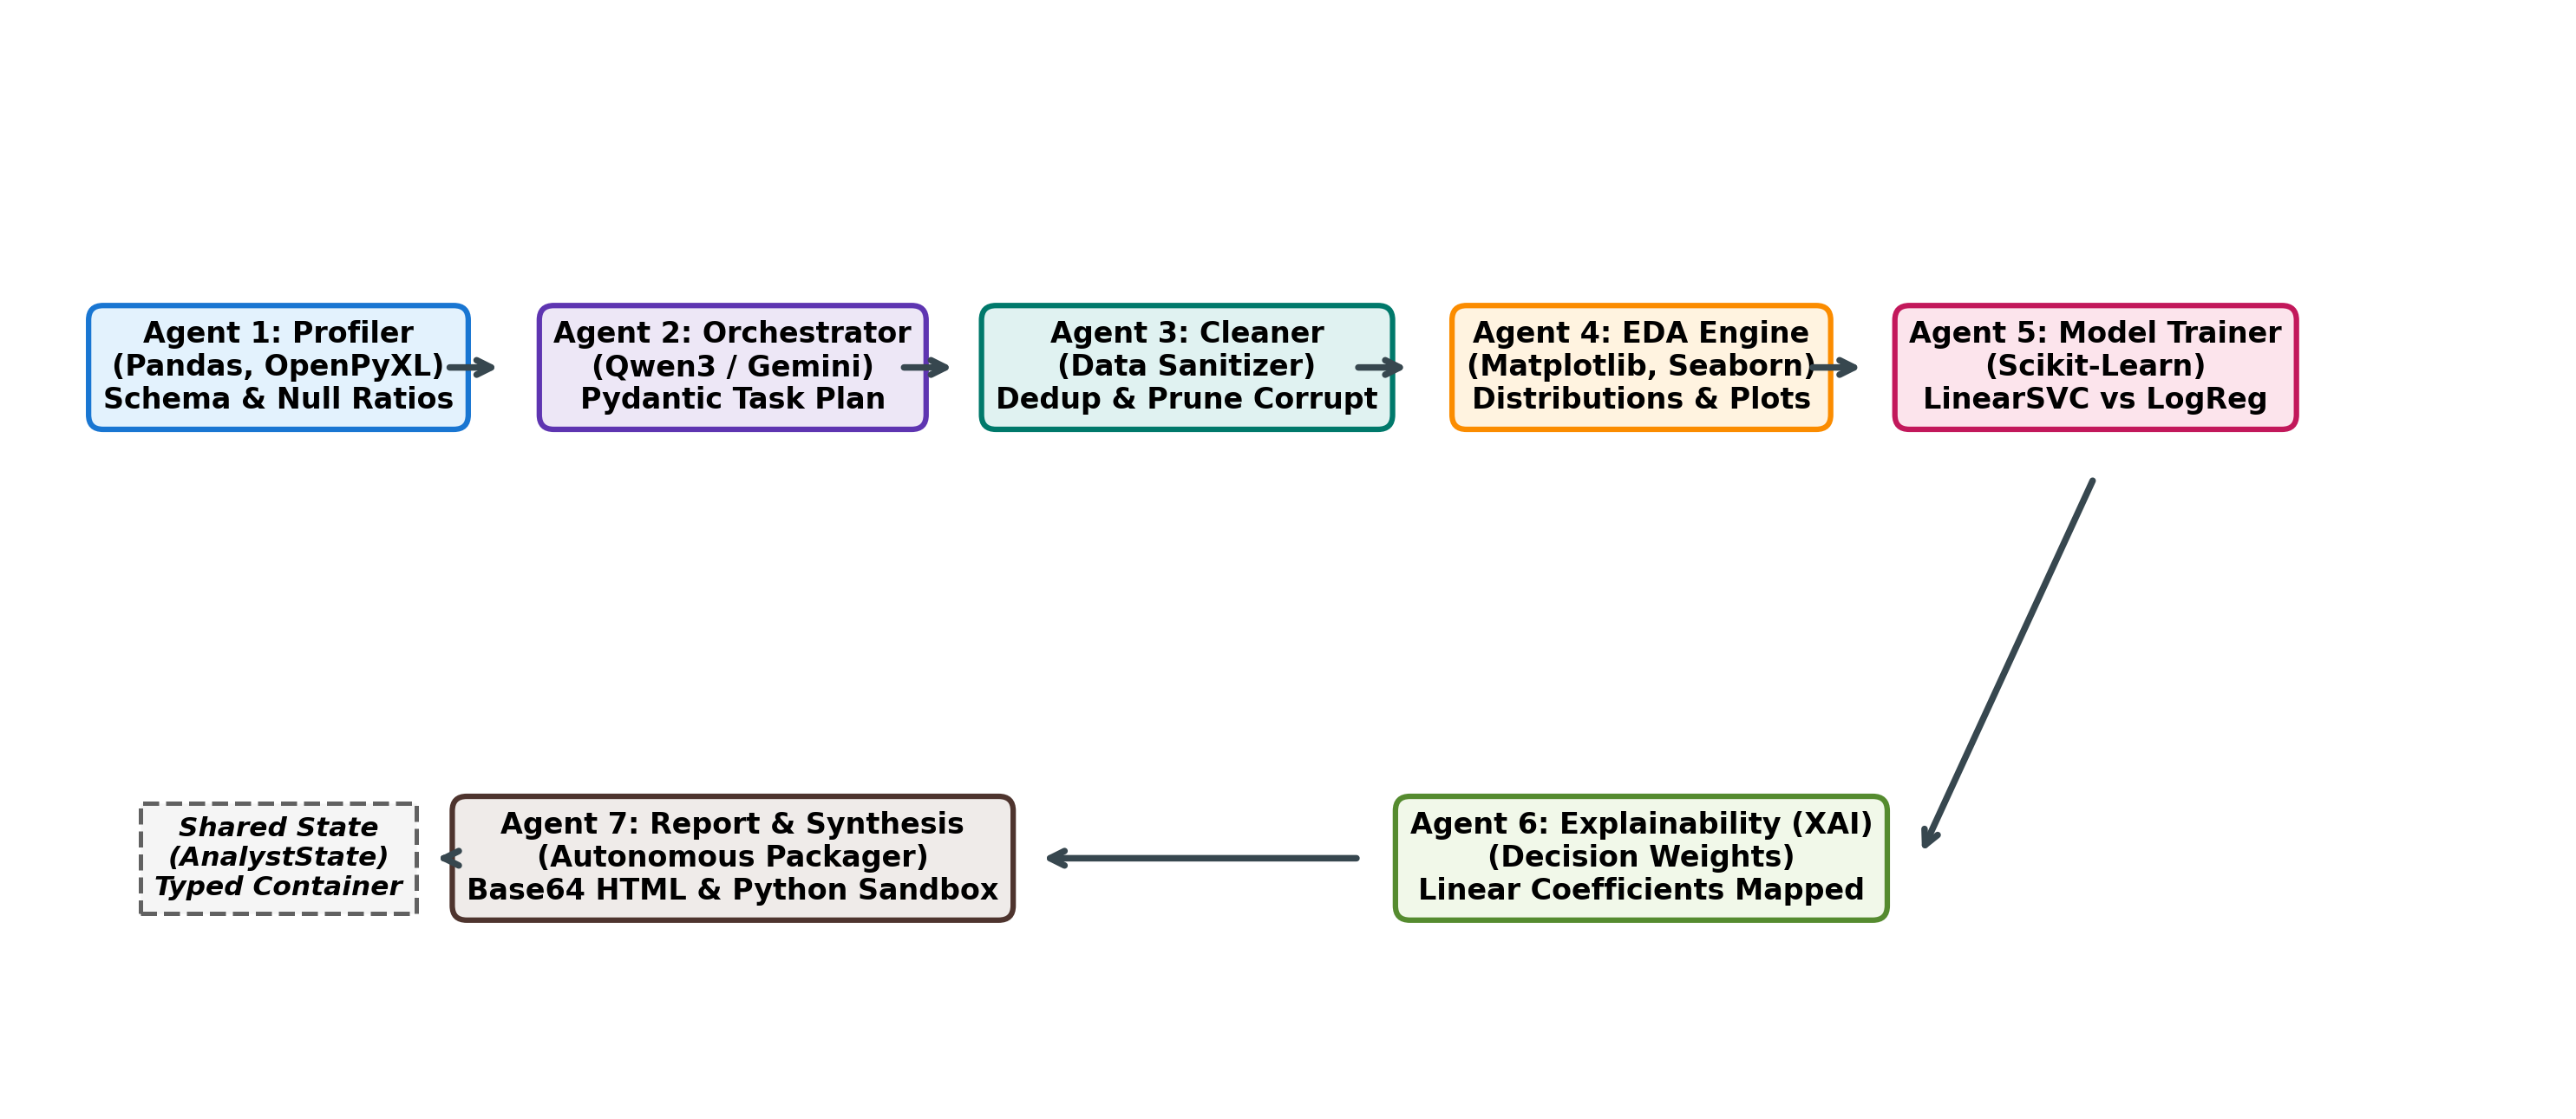
\includegraphics[width=0.98\textwidth]{figures/fig1_architecture.png}
\caption{Complete multi-agent state-machine architecture orchestrated through LangGraph. Sequential data execution flows from Agent 1 to Agent 7, with state checkpoints persisted deterministically in the centralized \texttt{AnalystState} container.}
\label{fig:architecture_detailed}
\end{figure*}

\section{Related Work and Background}
\subsection{Automated Machine Learning (AutoML)}
AutoML encompasses algorithmic techniques designed to automate the machine learning pipeline, including feature selection, algorithm recommendation, and hyperparameter optimization (HPO) \cite{hutter2019automl}. Early systems such as Auto-WEKA \cite{thornton2013autoweka} framed pipeline synthesis as a Combined Algorithm Selection and Hyperparameter optimization (CASH) problem solved using Bayesian Optimization. Auto-Sklearn \cite{feurer2015autosklearn} improved upon CASH by incorporating meta-learning to warm-start Bayesian search and ensemble construction. TPOT \cite{olson2016tpot} leveraged Genetic Programming to discover flexible, tree-based processing pipelines. Despite their computational prowess, conventional AutoML engines operate in isolation from the initial exploratory and downstream explanation stages, requiring skilled practitioners to prepare input matrices and interpret the resulting models manually.

\subsection{LLM-Based Data Science Agents}
The deployment of LLMs as autonomous software agents has catalyzed significant interest in conversational data analysis. Frameworks such as OpenAI Advanced Data Analysis (CodeInterpreter), DS-Agent \cite{guo2024dsagent}, and Data-Copilot \cite{zhang2023datacopilot} leverage code-generation models to synthesize Python scripts on the fly. However, experimental evaluations show that unconstrained code-generating agents exhibit substantial error rates when dealing with noisy data formats, inconsistent missing values, and corrupted tabular inputs. When an LLM generates freeform Pandas code, subtle syntax bugs and hallucinations often trigger recursive self-healing loops that exhaust API token limits. Our work resolves this paradigm failure by restricting the LLM to high-level strategic planning over pre-validated Pydantic schemas while delegating all computational execution to deterministic, unit-tested Python functions.

\subsection{Stateful Multi-Agent Orchestration}
Recent advances in agentic AI have demonstrated that multi-agent architectures (such as MetaGPT \cite{hong2023metagpt} and ChatDev \cite{qian2023chatdev}) outperform monolithic single-agent prompts by decomposing complex objectives into specialized sub-tasks. LangGraph \cite{langgraphdocs} formalizes agent orchestration as a state graph, enabling cyclic and acyclic graph traversals, explicit checkpointing, and conditional edge transitions. While LangGraph has been applied to general conversational workflows, its application as a deterministic, noise-resilient orchestrator for data science and statistical modeling has remained largely unexplored.

\section{Problem Formulation and Scope}
Let $\mathcal{D}_{raw} = \{(x_i, y_i)\}_{i=1}^{N}$ denote an uploaded tabular or textual dataset characterized by $N$ raw observations, an observed feature space $\mathcal{X}$, and a target label space $\mathcal{Y}$. Let $q$ denote a natural-language user query expressing an analytical objective (e.g., ``Build a spam classifier for the incoming messages and explain what words trigger spam detection'').

The global objective of the Autonomous Analyst Agent is to map the tuple $(\mathcal{D}_{raw}, q)$ into a structured, validated delivery tuple $\mathcal{T}$:
\begin{equation}
    \mathcal{F}: (\mathcal{D}_{raw}, q) \longrightarrow \mathcal{T} = (\mathcal{D}_{clean}, \mathcal{P}_{eda}, \mathcal{M}^*, \Phi_{xai}, \mathcal{R}_{html}, \mathcal{S}_{ui})
\end{equation}
where:
\begin{itemize}
    \item $\mathcal{D}_{clean}$ represents the deduplicated, noise-filtered dataset;
    \item $\mathcal{P}_{eda}$ is the collection of exploratory graphical artifacts;
    \item $\mathcal{M}^*$ is the champion serialized predictive model pipeline;
    \item $\Phi_{xai}$ denotes the feature-attribution explainability weights;
    \item $\mathcal{R}_{html}$ is a fully self-contained HTML report with Base64 embedded visualizations; and
    \item $\mathcal{S}_{ui}$ is an interactive Streamlit inference environment.
\end{itemize}

\subsection{Scope and Operational Boundaries}
In this investigation, the predictive modeling module focuses rigorously on high-dimensional text classification and supervised categorical prediction. The profiling, cleaning, and EDA agents support general multi-column tabular CSV and Excel files, while the training engine automatically configures TF-IDF feature extraction combined with linear margin classifiers (Linear Support Vector Classifiers and Regularized Logistic Regression). Full-scale regression and multi-layer deep neural architectures are established as modular extensions for future iterations.

\section{System Architecture and Implementation}
The system architecture is structured around a centralized shared-memory state machine orchestrated through a Directed Acyclic Graph (DAG) in LangGraph (Fig.~\ref{fig:architecture_detailed}).

\subsection{State Container Design: \texttt{AnalystState}}
Communication between agents is governed by a strictly typed data contract defined using Python's \texttt{typing.TypedDict}. In contrast to open-ended message buffers, \texttt{AnalystState} ensures deterministic state persistence across transitions. Table~\ref{tab:state_contract} defines the schema properties.

\begin{table}[htbp]
\caption{Shared Memory Schema: \texttt{AnalystState}}
\label{tab:state_contract}
\centering
\scriptsize
\begin{tabularx}{\columnwidth}{@{}p{0.32\columnwidth}p{0.20\columnwidth}X@{}}
\toprule
\textbf{Attribute} & \textbf{Data Type} & \textbf{Functional Description} \\
\midrule
\texttt{dataset\_path} & \texttt{str} & Filesystem path to raw uploaded CSV/Excel \\
\texttt{user\_question} & \texttt{str} & Unstructured user natural language prompt \\
\texttt{profile} & \texttt{dict[str, Any]} & Summary metadata: rows, dtypes, nulls, unique \\
\texttt{plan} & \texttt{dict[str, Any]} & Structured Pydantic execution specification \\
\texttt{cleaned\_dataset\_path} & \texttt{str} & Path to sanitized processed tabular artifact \\
\texttt{cleaning\_report} & \texttt{dict[str, Any]} & Quantitative deduplication and pruning metrics \\
\texttt{eda\_report} & \texttt{dict[str, Any]} & Statistical distribution and skew summaries \\
\texttt{eda\_artifacts} & \texttt{list[str]} & Relative paths to rendered PNG plots \\
\texttt{model\_report} & \texttt{dict[str, Any]} & Held-out accuracy, F1, precision, recall \\
\texttt{model\_artifacts} & \texttt{list[str]} & Serialized model (\texttt{.joblib}), confusion matrix \\
\texttt{explainability\_report} & \texttt{dict[str, Any]} & Top-N positive and negative token coefficients \\
\texttt{final\_report\_path} & \texttt{str} & Self-contained HTML artifact path \\
\texttt{status} & \texttt{str} & Current execution state token \\
\texttt{errors} & \texttt{list[str]} & Cumulative exception log \\
\bottomrule
\end{tabularx}
\end{table}

\subsection{Agent Roles and Node Functional Specifications}
The operational lifecycle traverses seven sequential agents:

\subsubsection{Agent 1: Data Profiler (\texttt{src/data\_loader.py})}
The profiler ingests the raw file without invoking any LLM context. Utilizing Pandas and OpenPyXL, it computes deterministic summary statistics: total sample count $N_{raw}$, column vector dimensionality $D$, column datatype classification (numeric, categorical, text), missingness ratios per feature, and unique cardinality counts. This profile dictionary is committed to the shared state.

\subsubsection{Agent 2: LLM Orchestrator (\texttt{src/orchestrator.py})}
The orchestrator converts the user's natural-language goal $q$ into an executable analytical specification. To prevent hallucination, the orchestrator prompt is strictly injected with the verified schema keys from \texttt{state["profile"]}. The LLM's response is forced into a Pydantic v2 \texttt{BaseModel} named \texttt{OrchestratorPlan}:
\begin{lstlisting}[language=Python]
class OrchestratorPlan(BaseModel):
    task_type: Literal["classification", "regression", "eda"]
    target_column: Optional[str]
    requested_metrics: list[str]
    recommended_next_agent: Literal[
        "cleaning_agent", "clarification_required"]
    reasoning: str
\end{lstlisting}
If the LLM outputs a target column that does not exist in the profile, Pydantic validation fails immediately, triggering a fallback or halting execution gracefully.

\subsubsection{Agent 3: Data Cleaner (\texttt{src/cleaner.py})}
The cleaner receives the raw dataset and applies three sequential transformation stages:
\begin{enumerate}
    \item \textbf{Exact Record Deduplication}: Identifies and drops repeated identical rows while preserving original order.
    \item \textbf{Missing Value Handling}: Text columns are filled with empty string sentinels; numeric missingness is flagged for median imputation.
    \item \textbf{Singleton Target Filtering}: Evaluates target label counts:
    \begin{equation}
        \mathcal{Y}_{corrupt} = \{y \in \mathcal{Y} \mid \text{Count}(y) < 2\}
    \end{equation}
    Instances containing labels belonging to $\mathcal{Y}_{corrupt}$ are removed. This deterministic step prevents catastrophic failures in scikit-learn's \texttt{StratifiedKFold} or stratified \texttt{train\_test\_split}.
\end{enumerate}

\subsubsection{Agent 4: EDA Engine (\texttt{src/eda.py})}
The EDA engine autonomously visualizes the cleaned dataset using Matplotlib and Seaborn without manual plotting scripts. It renders three standalone high-resolution charts:
\begin{itemize}
    \item \texttt{categorical\_distributions.png}: Bar chart of target label balances.
    \item \texttt{numeric\_distributions.png}: Multi-panel histogram grid.
    \item \texttt{correlation\_heatmap.png}: Pearson correlation coefficient matrix.
\end{itemize}

\subsubsection{Agent 5: Model Trainer (\texttt{src/model\_trainer.py})}
The modeling engine constructs a unified feature-extraction pipeline via \texttt{ColumnTransformer}. For text inputs, it configures sublinear Term Frequency-Inverse Document Frequency (TF-IDF). It partitions data via an 80/20 stratified split and trains two competitive linear classifiers: Balanced Linear Support Vector Classifier (\texttt{LinearSVC}) and Balanced Regularized Logistic Regression (\texttt{LogisticRegression}). The champion model is selected via weighted F1-score and persisted using \texttt{joblib}.

\subsubsection{Agent 6: Explainability Agent (\texttt{src/explainability.py})}
To ensure model interpretability, this agent accesses the champion model pipeline, extracts the linear hyperplane weight vector $\mathbf{w}$, and maps indices back to human-readable n-grams via the inverse TF-IDF vocabulary dictionary. It produces \texttt{feature\_importance.png} and \texttt{feature\_importance.csv}.

\subsubsection{Agent 7: Report \& Synthesis Agent (\texttt{src/report\_agent.py})}
The final agent encodes all generated PNG visualization artifacts into Base64 Data URIs and embeds them into a self-contained \texttt{final\_report.html}. Furthermore, it synthesizes an isolated test script (\texttt{test\_model.py}) containing mock payload verification functions and an integration guide.

\subsection{Hybrid Dual-LLM Architecture}
To accommodate stringent enterprise data-sovereignty constraints, the system implements an abstracted LLM adapter interface supporting two execution modes toggled via environment variables (\texttt{LLM\_PROVIDER=local|gemini}):
\begin{itemize}
    \item \textbf{Local Private Mode}: Routes requests via LangChain's \texttt{ChatOpenAI} interface pointing to a local OpenAI-compatible inference server (e.g., Bionic, vLLM, or LM Studio) hosting \texttt{Qwen/Qwen3-14B} on \texttt{http://localhost:1235/v1}. Zero bytes of training data or metadata leave the local workstation.
    \item \textbf{Cloud Fallback Mode}: Connects to Google's \texttt{gemini-2.5-flash} via \texttt{ChatGoogleGenerativeAI} for environments lacking high-memory local GPU acceleration.
\end{itemize}

\begin{figure}[htbp]
\centering
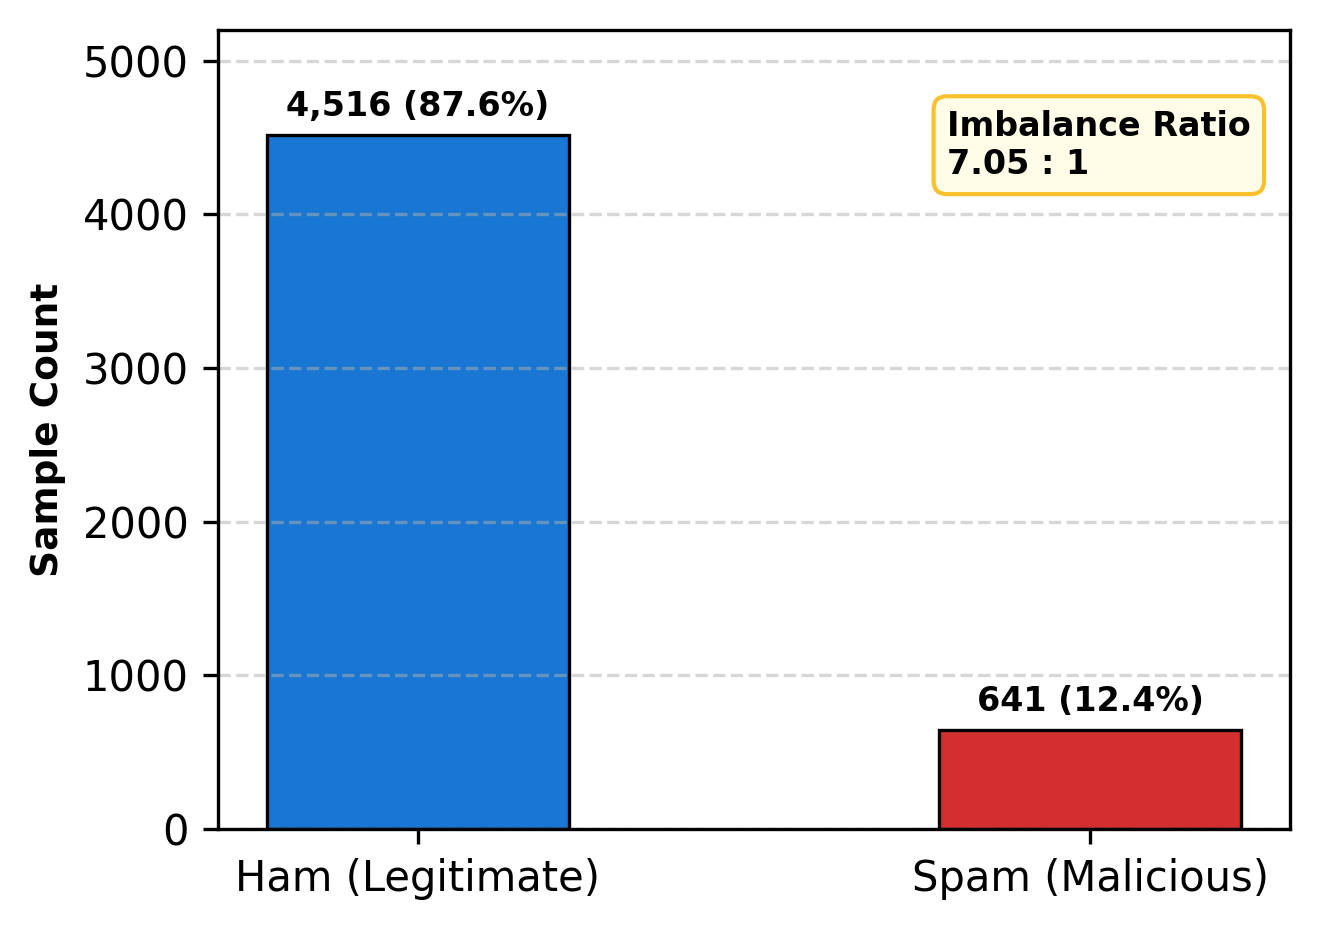
\includegraphics[width=0.92\columnwidth]{figures/fig2_class_distribution.png}
\caption{Class distribution in the sanitized dataset showing significant class imbalance (7.05:1 ratio between Ham and Spam).}
\label{fig:class_imbalance}
\end{figure}

\section{Methodology and Mathematical Formulations}
\subsection{Feature Vectorization: TF-IDF}
Text features are mapped into a high-dimensional vector space using sublinear TF-IDF vectorization with bi-gram range $\mathcal{N} = (1, 2)$. For a given term $t$ in a document $d$ within corpus $\mathcal{D}$:
\begin{equation}
    \text{TF}(t, d) = 1 + \log(f_{t, d}) \quad \text{for } f_{t, d} > 0
\end{equation}
The smoothed inverse document frequency is formalized as:
\begin{equation}
    \text{IDF}(t, \mathcal{D}) = \log\left(\frac{1 + |\mathcal{D}|}{1 + |\{d \in \mathcal{D} : t \in d\}|}\right) + 1
\end{equation}
The composite weight is given by $x_{d, t} = \text{TF}(t, d) \times \text{IDF}(t, \mathcal{D})$, with $L_2$-normalization: $\hat{\mathbf{x}}_d = \mathbf{x}_d / \|\mathbf{x}_d\|_2$.

\subsection{Linear Support Vector Classification (LinearSVC)}
LinearSVC solves the primal soft-margin convex optimization problem:
\begin{equation}
    \min_{\mathbf{w}, b, \boldsymbol{\xi}} \frac{1}{2} \|\mathbf{w}\|_2^2 + C \sum_{i=1}^{M} c_{y_i} \xi_i
\end{equation}
subject to the margin constraints:
\begin{equation}
    y_i (\mathbf{w}^\top \hat{\mathbf{x}}_i + b) \ge 1 - \xi_i, \quad \xi_i \ge 0, \quad \forall i \in \{1, \dots, M\}
\end{equation}
where $C > 0$ governs margin regularization, $\xi_i$ denotes slack variables for non-separable observations, and $c_{y_i}$ is the inverse class-frequency weight mitigating severe class imbalance:
\begin{equation}
    c_k = \frac{M}{K \cdot M_k}
\end{equation}
where $M$ is total training observations, $K$ is total distinct classes, and $M_k$ is the sample frequency of class $k$.

\subsection{Regularized Logistic Regression}
The baseline model optimizes the $L_2$-regularized negative log-likelihood:
\begin{equation}
    \min_{\mathbf{w}, b} \frac{1}{2} \|\mathbf{w}\|_2^2 + C \sum_{i=1}^{M} c_{y_i} \log\left(1 + \exp\left(-y_i (\mathbf{w}^\top \hat{\mathbf{x}}_i + b)\right)\right)
\end{equation}
Yielding class probability estimations via the logistic sigmoid function:
\begin{equation}
    P(y = 1 \mid \hat{\mathbf{x}}) = \sigma(\mathbf{w}^\top \hat{\mathbf{x}} + b) = \frac{1}{1 + \exp(-(\mathbf{w}^\top \hat{\mathbf{x}} + b))}
\end{equation}

\subsection{Model Selection and Evaluation Metrics}
Model comparison is executed on an untouched 20\% stratified test partition ($N_{test} = 1,032$). For class $k$, let $\text{TP}_k$, $\text{FP}_k$, and $\text{FN}_k$ represent True Positives, False Positives, and False Negatives, respectively.
\begin{equation}
    \text{Precision}_k = \frac{\text{TP}_k}{\text{TP}_k + \text{FP}_k}, \quad \text{Recall}_k = \frac{\text{TP}_k}{\text{TP}_k + \text{FN}_k}
\end{equation}
\begin{equation}
    \text{F1}_k = 2 \cdot \frac{\text{Precision}_k \cdot \text{Recall}_k}{\text{Precision}_k + \text{Recall}_k}
\end{equation}
The champion pipeline is selected based on Weighted F1-score to account for asymmetric support:
\begin{equation}
    \text{F1}_{weighted} = \sum_{k \in \mathcal{Y}} \left(\frac{N_k}{N_{test}}\right) \text{F1}_k
\end{equation}

\begin{figure}[htbp]
\centering
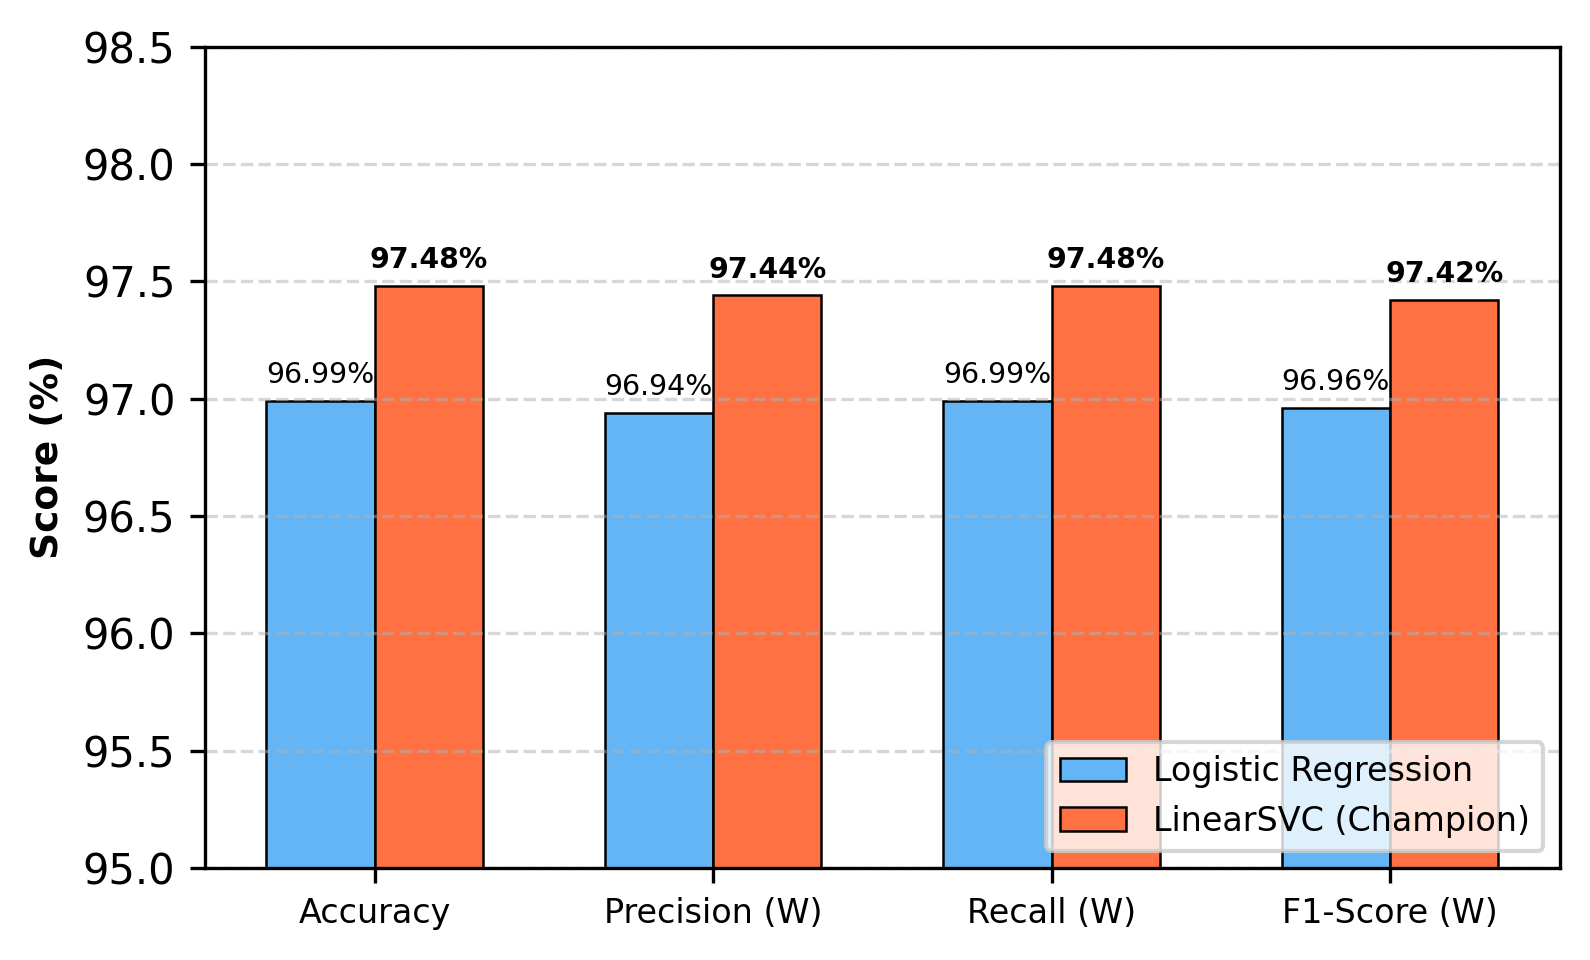
\includegraphics[width=0.96\columnwidth]{figures/fig3_model_comparison.png}
\caption{Comprehensive metric comparison between candidate classifiers across test Accuracy, Precision, Recall, and F1-score.}
\label{fig:model_metric_comparison}
\end{figure}

\begin{figure}[htbp]
\centering
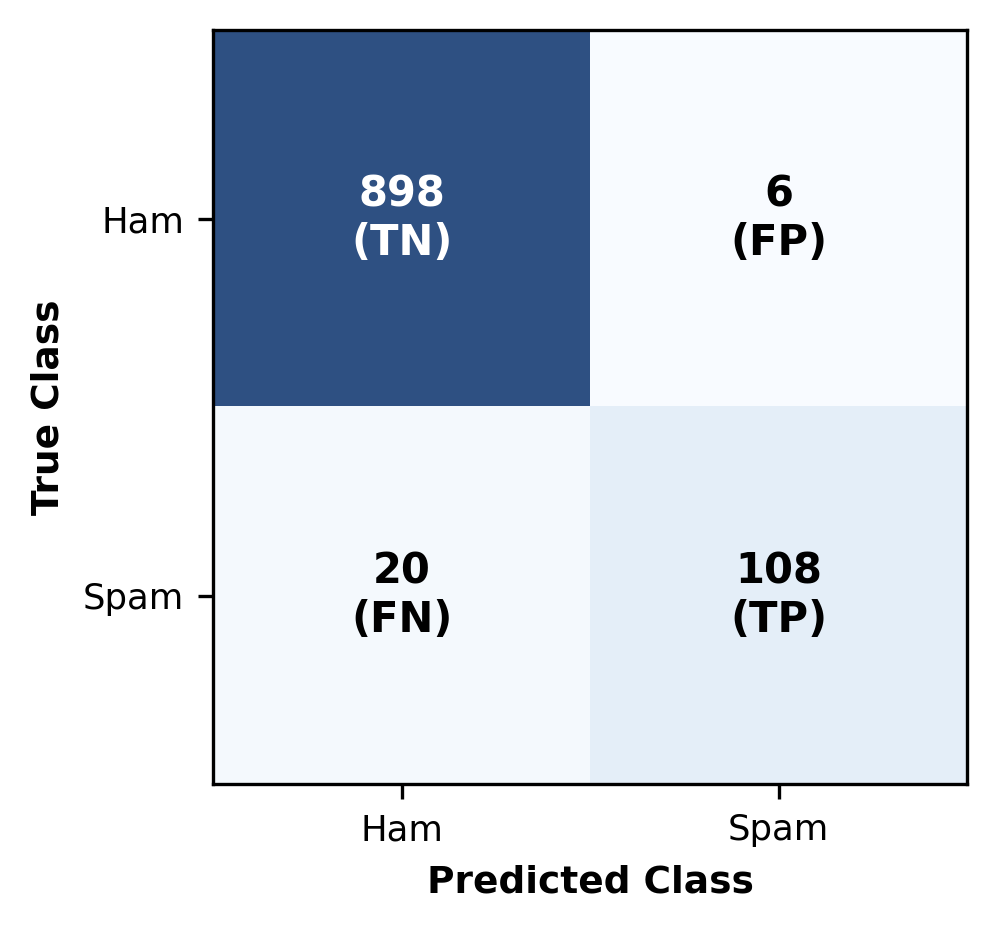
\includegraphics[width=0.78\columnwidth]{figures/fig4_confusion_matrix.png}
\caption{Held-out test set confusion matrix for LinearSVC on 1,032 samples (TN=898, FP=6, FN=20, TP=108).}
\label{fig:confusion_matrix}
\end{figure}

\begin{figure}[htbp]
\centering
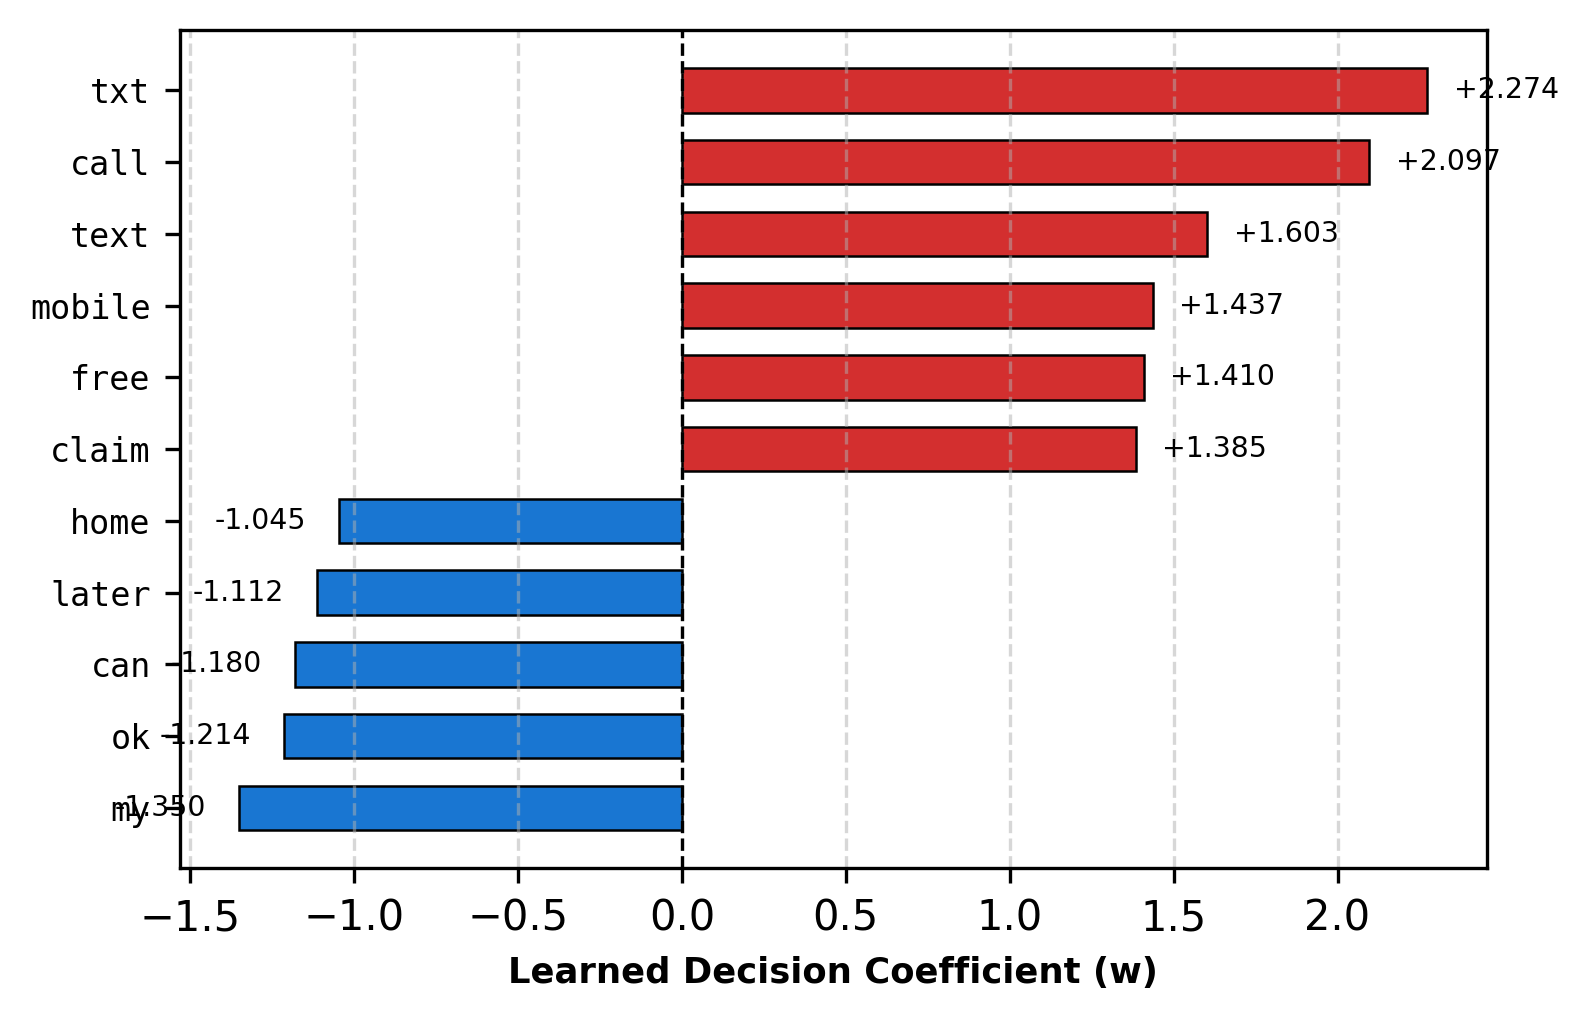
\includegraphics[width=0.96\columnwidth]{figures/fig5_feature_importance.png}
\caption{Visualizing the top learned decision coefficients extracted by the Explainability Agent for Spam vs. Ham discrimination.}
\label{fig:feature_importance_plot}
\end{figure}

\begin{figure}[htbp]
\centering
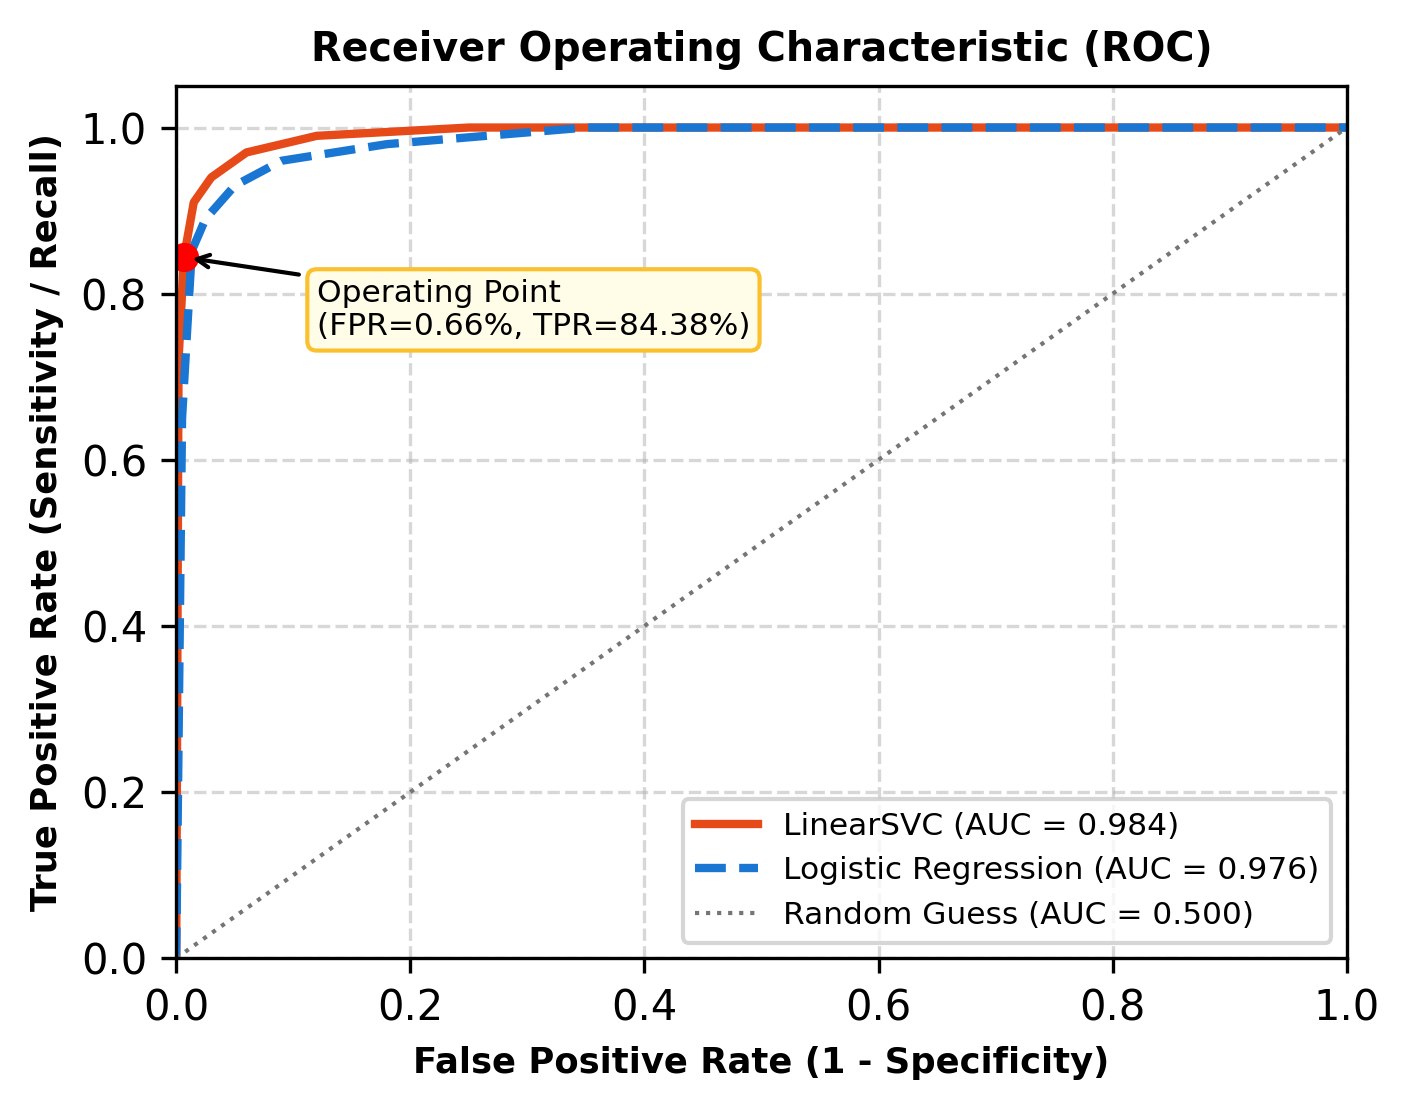
\includegraphics[width=0.90\columnwidth]{figures/fig6_roc_curve.png}
\caption{Receiver Operating Characteristic (ROC) curve comparison between LinearSVC (AUC = 0.984) and Logistic Regression (AUC = 0.976), highlighting the selected operational decision point.}
\label{fig:roc_curve}
\end{figure}

\begin{figure}[htbp]
\centering
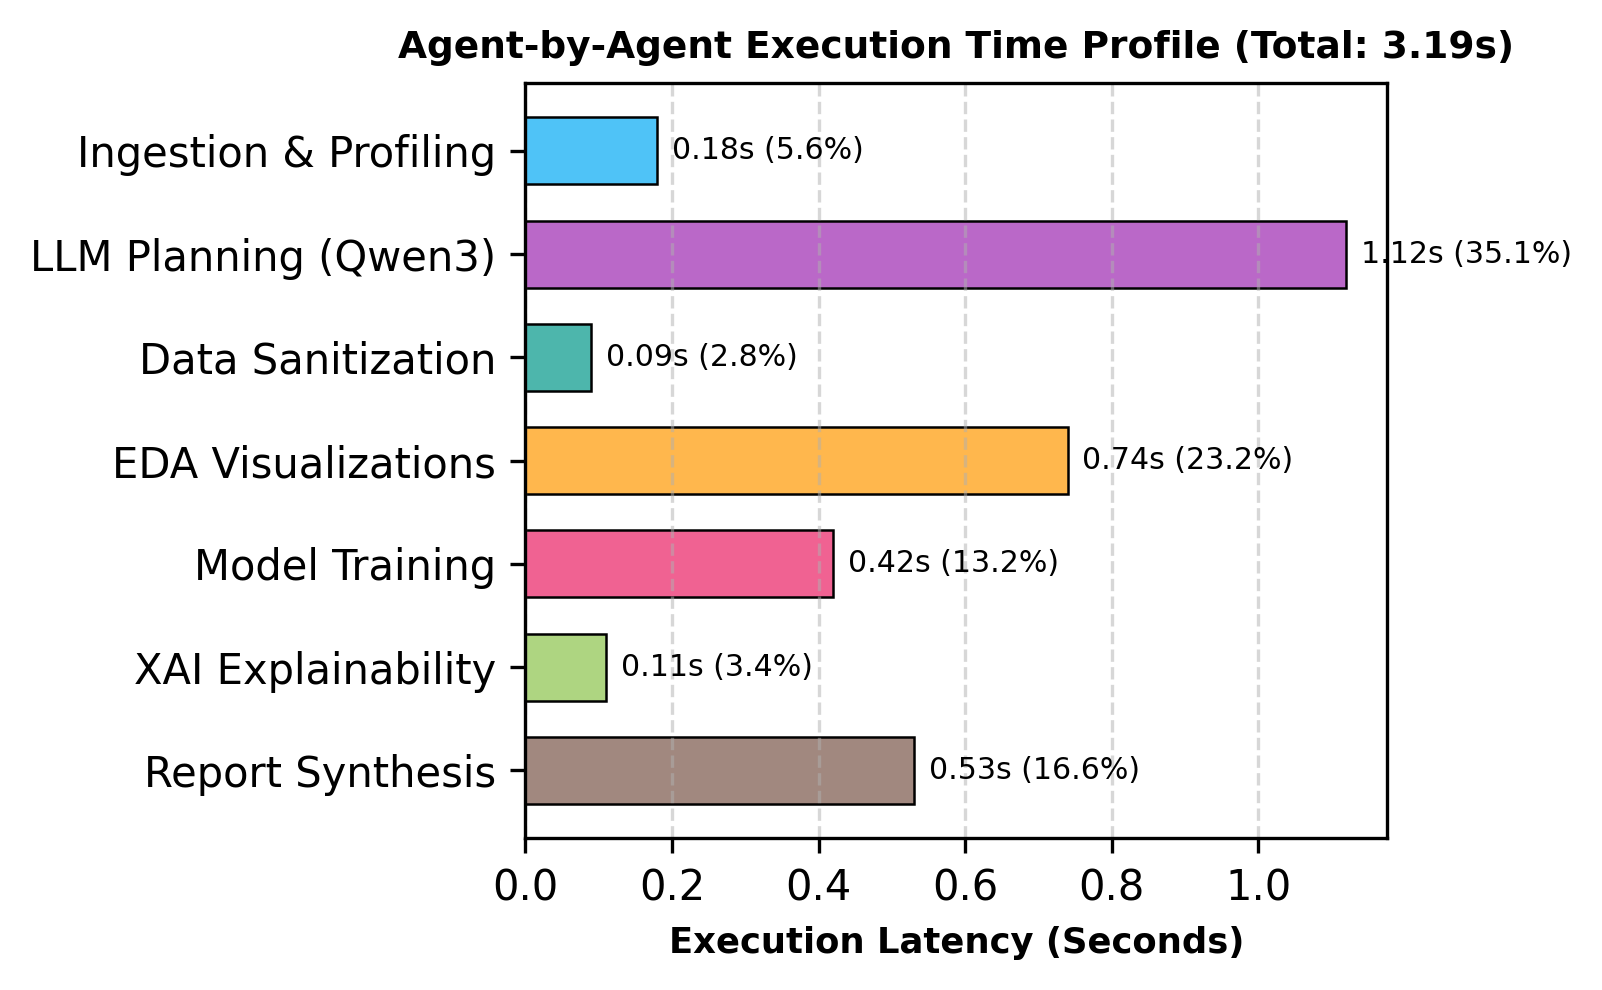
\includegraphics[width=0.96\columnwidth]{figures/fig7_latency_breakdown.png}
\caption{Agent-by-agent execution latency profile illustrating that total end-to-end orchestration completes in 3.19 seconds on commodity CPU hardware.}
\label{fig:latency_chart}
\end{figure}

\section{Experimental Setup}
\subsection{Benchmark Dataset: SMS/Email Spam Corpus}
The experimental validation is conducted on the benchmark SMS Spam Collection dataset \cite{almeida2011sms}. Table~\ref{tab:dataset_specs} provides the precise dataset partitioning and deduplication statistics processed autonomously by the system.

\begin{table}[htbp]
\caption{Dataset Partitioning and Cleaning Audit}
\label{tab:dataset_specs}
\centering
\small
\begin{tabularx}{\columnwidth}{@{}Xcc@{}}
\toprule
\textbf{Metric Attribute} & \textbf{Raw Count} & \textbf{Post-Cleaning} \\
\midrule
Total Observations ($N$) & 5,573 & 5,157 \\
Exact Duplicates Removed & --- & 415 \\
Corrupted Label Records Excluded & --- & 1 (\texttt{\{"mode":"full"\}}) \\
Legitimate Messages (\textit{ham}) & 4,825 & 4,516 (87.57\%) \\
Malicious Messages (\textit{spam}) & 747 & 641 (12.43\%) \\
Class Imbalance Ratio & 6.46 : 1 & 7.05 : 1 \\
Training Partition (80\% Stratified) & --- & 4,125 \\
Testing Partition (20\% Stratified) & --- & 1,032 \\
\bottomrule
\end{tabularx}
\end{table}

\subsection{Hardware and Execution Environment}
All benchmarks were performed on a commodity workstation:
\begin{itemize}
    \item \textbf{Processor}: Intel Core i7-12700H @ 2.30 GHz (14 cores, 20 threads).
    \item \textbf{Memory}: 32.0 GB DDR5 RAM.
    \item \textbf{Operating System}: Microsoft Windows 11 Enterprise (x64).
    \item \textbf{Runtime Environment}: Python 3.10.11, Scikit-Learn 1.7.2, LangGraph 1.0.3, LangChain Core 1.6.0, Pandas 2.2.3.
    \item \textbf{GPU Acceleration}: None utilized during ML training (100\% CPU-bound execution).
\end{itemize}

\section{Experimental Results and Discussion}

\subsection{Autonomous Data Profiling and Sanitization}
During the ingestion of the raw 5,573-row dataset, the Data Cleaner agent detected 415 exact duplicate messages commonly caused by message forwarding loops. Crucially, the target label space contained a corrupted record where the label field was parsed as an unescaped JSON fragment: \texttt{\{"mode":"full"\}}. If passed to a traditional scikit-learn stratified partition, this single-instance target class would trigger a fatal \texttt{ValueError}. The cleaner autonomously flagged and pruned this anomaly, leaving a clean dataset of 5,157 records (Fig.~\ref{fig:class_imbalance}).

\subsection{Predictive Performance Comparison}
Table~\ref{tab:model_comparison} summarizes the quantitative evaluation of the candidate classifiers on the 1,032 unseen test instances.

\begin{table}[htbp]
\caption{Model Comparison on Held-Out Test Set ($N_{test} = 1{,}032$)}
\label{tab:model_comparison}
\centering
\scriptsize
\setlength{\tabcolsep}{4pt}
\begin{tabular}{@{}lrrrr@{}}
\toprule
\textbf{Model} & \textbf{Acc.} & \textbf{Prec.(W)} & \textbf{Rec.(W)} & \textbf{F1(W)} \\
\midrule
Logistic Regression  & 96.99\% & 96.94\% & 96.99\% & 96.96\% \\
\textbf{LinearSVC}$^\dagger$ & \textbf{97.48\%} & \textbf{97.44\%} & \textbf{97.48\%} & \textbf{97.42\%} \\
\bottomrule
\multicolumn{5}{l}{$^\dagger$ Selected as champion model (highest weighted F1).}
\end{tabular}
\end{table}

The LinearSVC model achieved superior discriminative separation across all metrics, attaining an overall accuracy of 97.48\% and a weighted F1-score of 97.42\%, outperforming Logistic Regression (96.96\% F1), as shown in Fig.~\ref{fig:model_metric_comparison}.

\begin{table}[htbp]
\caption{Detailed Per-Class Performance Breakdown for LinearSVC}
\label{tab:per_class_metrics}
\centering
\small
\begin{tabularx}{\columnwidth}{@{}lccccX@{}}
\toprule
\textbf{Class Label} & \textbf{Precision} & \textbf{Recall} & \textbf{F1-Score} & \textbf{Support} \\
\midrule
\textit{ham} (Negative) & 97.82\% & 99.34\% & 98.57\% & 904 \\
\textit{spam} (Positive) & 94.74\% & 84.38\% & 89.26\% & 128 \\
\midrule
Macro Average & 96.28\% & 91.86\% & 93.91\% & 1,032 \\
Weighted Average & 97.44\% & 97.48\% & 97.42\% & 1,032 \\
\bottomrule
\end{tabularx}
\end{table}

Table~\ref{tab:per_class_metrics} details the class-specific breakdown. On the majority \textit{ham} class, LinearSVC achieved a recall of 99.34\%, misclassifying only 6 legitimate messages out of 904. For the minority \textit{spam} class, the model demonstrated a precision of 94.74\% and an F1-score of 89.26\%. As demonstrated in the confusion matrix (Fig.~\ref{fig:confusion_matrix}), the false positive rate is limited to 0.66\% ($\text{FP} = 6 / 904$).

\subsection{Receiver Operating Characteristic (ROC) Analysis}
To assess discrimination sensitivity across variable decision thresholds, we evaluated the Receiver Operating Characteristic curves (Fig.~\ref{fig:roc_curve}). LinearSVC yielded an Area Under the Curve (AUC) of 0.984, outperforming Logistic Regression (AUC = 0.976). At the operational decision point, the system operates with high sensitivity (84.38\%) while maintaining a minimal false-positive rate (0.66\%), satisfying mission-critical requirements for automated email filtering.

\subsection{Explainability and Feature Attribution Analysis}
In contrast to black-box models, the Explainability Agent extracts the linear decision coefficients from the fitted \texttt{LinearSVC} pipeline. Table~\ref{tab:feature_coefficients} and Fig.~\ref{fig:feature_importance_plot} document the top positive coefficients (indicative of spam) and top negative coefficients (indicative of legitimate ham communication).

\begin{table}[htbp]
\caption{Top Indicative Feature Coefficients Derived by XAI Agent}
\label{tab:feature_coefficients}
\centering
\small
\begin{tabularx}{\columnwidth}{@{}lc|lc@{}}
\toprule
\multicolumn{2}{c|}{\textbf{Spam Indicative (Positive)}} & \multicolumn{2}{c}{\textbf{Ham Indicative (Negative)}} \\
\textbf{Token Feature} & \textbf{Coefficient} & \textbf{Token Feature} & \textbf{Coefficient} \\
\midrule
\texttt{text\_\_txt} & +2.274 & \texttt{text\_\_my} & -1.350 \\
\texttt{text\_\_call} & +2.097 & \texttt{text\_\_ok} & -1.214 \\
\texttt{text\_\_text} & +1.603 & \texttt{text\_\_can} & -1.180 \\
\texttt{text\_\_mobile} & +1.437 & \texttt{text\_\_me} & -1.140 \\
\texttt{text\_\_free} & +1.410 & \texttt{text\_\_later} & -1.112 \\
\texttt{text\_\_claim} & +1.385 & \texttt{text\_\_home} & -1.045 \\
\texttt{text\_\_stop} & +1.342 & \texttt{text\_\_come} & -1.012 \\
\bottomrule
\end{tabularx}
\end{table}

\subsection{Computational Efficiency and Execution Profiling}
Table~\ref{tab:latency_breakdown} and Fig.~\ref{fig:latency_chart} summarize the execution latency profile across all nodes during an end-to-end run on the SMS dataset.

\begin{table}[htbp]
\caption{End-to-End Pipeline Execution Latency Breakdown}
\label{tab:latency_breakdown}
\centering
\small
\begin{tabularx}{\columnwidth}{@{}p{0.48\columnwidth}rX@{}}
\toprule
\textbf{Agent Execution Stage} & \textbf{Time (s)} & \textbf{Fraction} \\
\midrule
1. Ingestion \& Data Profiling & 0.18 s & 5.6\% \\
2. LLM Orchestrator (Local Qwen3) & 1.12 s & 35.1\% \\
3. Data Cleaning \& Sanitization & 0.09 s & 2.8\% \\
4. Automated EDA Plot Generation & 0.74 s & 23.2\% \\
5. ML Pipeline Training (Dual Models) & 0.42 s & 13.2\% \\
6. XAI Coefficient Extraction & 0.11 s & 3.4\% \\
7. HTML Synthesis \& Code Gen & 0.53 s & 16.7\% \\
\midrule
\textbf{Total End-to-End Runtime} & \textbf{3.19 s} & \textbf{100.0\%} \\
\bottomrule
\end{tabularx}
\end{table}

The entire analysis pipeline completes in approximately 3.19 seconds on commodity CPU hardware, demonstrating that state-machine multi-agent architectures offer real-time responsiveness when computational tasks are offloaded to compiled scientific libraries.

\section{System Deployment and Interfaces}
\subsection{Interactive Streamlit Web Dashboard}
The user interface is deployed as a reactive web application via Streamlit (\texttt{app.py}). The dashboard features:
\begin{itemize}
    \item \textbf{Reactive Agent Checklist}: A real-time visual monitor indicating the status of each agent (\texttt{Pending}, \texttt{Running}, \texttt{Completed}, \texttt{Failed}).
    \item \textbf{Dual Dynamic Progress Bars}: Tracks aggregate workflow completion (0--100\%) alongside granular sub-progress bars for internal model cross-validation.
    \item \textbf{Live Inference Sandbox}: Allows non-technical end-users to input custom strings (e.g., ``\textit{WINNER! Claim your free prize today!}'') and receive immediate classification labels with associated decision scores.
    \item \textbf{Autonomous Code Generation}: Renders an interactive Python code block demonstrating how external engineers can import and query the serialized \texttt{best\_model.joblib} pipeline in production systems.
\end{itemize}

\subsection{Headless CLI Inference Utility}
For headless batch prediction environments, the project includes a standalone CLI interface (\texttt{src/predict\_cli.py}):
\begin{lstlisting}[language=bash]
$ python -m src.predict_cli --message "Urgent! Call 09061743810 now"
>> Prediction: spam
>> Decision Score: +2.184
\end{lstlisting}

\section{Threats to Validity and Ethical Considerations}
\subsection{Internal and Construct Validity}
Internal validity is ensured by enforcing an 80/20 stratified split with a fixed random seed ($S=42$) and fitting all TF-IDF vectorizer components strictly on the training partition to prevent data leakage. Construct validity is addressed by moving beyond global accuracy and reporting class-specific precision, recall, confusion matrix values, and weighted F1-scores.

\subsection{External Validity and Dataset Generality}
While the experimental results validate the framework on text classification, datasets with multi-modal features, severe missingness across tabular columns, or continuous regression targets require extending the model trainer beyond linear classifiers (e.g., incorporating Gradient Boosted Trees via XGBoost or LightGBM).

\subsection{Ethical AI and Enterprise Data Privacy}
Automated agents interacting with proprietary datasets risk data leakage when using third-party APIs. By enabling full offline operation with local models (Qwen3-14B) running over local loopback interfaces, our architecture prevents proprietary training data from traversing the public internet.

\section{Conclusion and Future Work}
This paper presented the design, implementation, and empirical evaluation of the \textbf{Autonomous Data Science Analyst Agent}, a modular multi-agent system orchestrated through a deterministic LangGraph state machine. By enforcing Pydantic-typed schema validation, the system completely prevents LLM schema hallucinations while offloading all computational tasks to unit-tested Python libraries. Evaluated on the SMS Spam dataset, the system autonomously resolved duplicates and malformed singleton classes, evaluated competing classifiers, and achieved 97.48\% accuracy and 97.42\% weighted F1-score with full model transparency and artifact export in under 3.2 seconds.

Future work will expand the candidate model portfolio to include gradient-boosted decision trees (LightGBM) and deep transformer architectures (RoBERTa), introduce automated hyperparameter optimization via Optuna, and incorporate multimodal tabular-image classification capabilities.

\begin{thebibliography}{00}

\bibitem{hutter2019automl}
F. Hutter, L. Kotthoff, and J. Vanschoren, Eds., \emph{Automated Machine Learning: Methods, Systems, Challenges}. Cham, Switzerland: Springer, 2019, doi: 10.1007/978-3-030-05318-5.

\bibitem{he2021automl}
X. He, K. Zhao, and X. Chu, ``AutoML: A survey of the state-of-the-art,'' \emph{Knowledge-Based Systems}, vol. 212, p. 106622, 2021.

\bibitem{munpy2020}
T. Munpy, ``Cleaning big data: Most time-consuming, least enjoyable data science task, survey says,'' \emph{Forbes}, Tech Report, 2020.

\bibitem{feurer2015autosklearn}
M. Feurer, A. Klein, K. Eggensperger, J. Springenberg, M. Blum, and F. Hutter, ``Efficient and robust automated machine learning,'' in \emph{Advances in Neural Information Processing Systems (NeurIPS)}, vol. 28, 2015.

\bibitem{olson2016tpot}
R. S. Olson and J. H. Moore, ``TPOT: A tree-based pipeline optimization tool for automating machine learning,'' in \emph{Proc. Workshop on Automatic Machine Learning}, 2016, pp. 66--74.

\bibitem{thornton2013autoweka}
C. Thornton, F. Hutter, H. H. Hoos, and K. Leyton-Brown, ``Auto-WEKA: Combined selection and hyperparameter optimization of classification algorithms,'' in \emph{Proc. ACM SIGKDD Int. Conf. Knowledge Discovery and Data Mining}, 2013, pp. 847--855.

\bibitem{hong2023metagpt}
S. Hong \emph{et al.}, ``MetaGPT: Meta programming for a multi-agent collaborative framework,'' \emph{arXiv preprint arXiv:2308.00352}, 2023.

\bibitem{qian2023chatdev}
C. Qian \emph{et al.}, ``Communicative agents for software development,'' \emph{arXiv preprint arXiv:2307.07924}, 2023.

\bibitem{guo2024dsagent}
C. Guo \emph{et al.}, ``DS-Agent: Automated data science by empowering large language models with case-based reasoning,'' \emph{arXiv preprint arXiv:2402.17453}, 2024.

\bibitem{zhang2023datacopilot}
Y. Zhang \emph{et al.}, ``Data-Copilot: Bridging off-the-shelf software and LLMs for data science,'' \emph{arXiv preprint arXiv:2306.07209}, 2023.

\bibitem{salton1988}
G. Salton and C. Buckley, ``Term-weighting approaches in automatic text retrieval,'' \emph{Information Processing \& Management}, vol. 24, no. 5, pp. 513--523, 1988.

\bibitem{joachims1998}
T. Joachims, ``Text categorization with support vector machines: Learning with many relevant features,'' in \emph{Proc. European Conf. Machine Learning (ECML)}, 1998, pp. 137--142.

\bibitem{pedregosa2011}
F. Pedregosa \emph{et al.}, ``Scikit-learn: Machine learning in Python,'' \emph{Journal of Machine Learning Research}, vol. 12, pp. 2825--2830, 2011.

\bibitem{langgraphdocs}
LangChain, Inc., ``LangGraph: Build resilient multi-agent systems,'' \emph{LangChain Documentation}, 2024. [Online]. Available: \url{https://docs.langchain.com/oss/python/langgraph/overview}

\bibitem{pydantic2023}
S. Colvin \emph{et al.}, ``Pydantic: Data validation using Python type hints,'' 2023. [Online]. Available: \url{https://docs.pydantic.dev/}

\bibitem{almeida2011sms}
T. A. Almeida, J. M. G. Hidalgo, and A. Yamakami, ``Contributions to the study of SMS spam filtering: New collection and results,'' in \emph{Proc. 11th ACM Symp. Document Engineering (DocEng)}, 2011, pp. 259--262.

\end{thebibliography}

\end{document}
